\documentclass[8pt]{report}
\usepackage{amsmath, xfrac, enumitem, graphicx, ulem, float, bigints, bm, textcomp}
\usepackage{titlesec, mathtools}
\usepackage[margin=0.7in]{geometry}
\graphicspath{ {images/} }
\linespread{0.8}
\title{\Huge{\textsc{Mathematics - GATE}}}
\author{\huge{\textbf{Kulasekaran}}}
\begin{document}
\maketitle
\tableofcontents
\chapter{Linear Algebra}
%-----------------------------------------------------------------------------------------%
\chapter{Differential and Integral Calculus}
%-----------------------------------------------------------------------------------------%
\chapter{Vector Calculus}
%-----------------------------------------------------------------------------------------%
\chapter{Differential Equations}
%-----------------------------------------------------------------------------------------%
\chapter{Probability}
\section{Introduction and Basics}
	\begin{itemize}
		\item \textbf{Random Experiment} : An experiment in which the result is unpredictable, but the possibilities of the result is known. Eg. When you throw a coin, you don't know its gonna be head or tail. But you know it will be either one of them.
		\item \textbf{Sample Space(S)} : A set of all possible outcomes of a random experiment is called its sample space. For the above mentioned coin toss example the sample space is s:\{H,T\} $\boxed{P(s)=1}$
		\item \textbf{Event} : A subset of the sample space is called as event. For the above mentioned example, the event can be in which the coin lands as H, or the event can be in which the coin lands as tail. Another example: Throwing a fair dice, S=\{1,2,3,4,5,6\}. An event can be in which the number on the top of the dice will be even, So $\implies$ \{2,4,6\}. $\boxed{0\le P(E)\le1}$
		\begin{itemize}
			\item \textbf{Simple event:} Only one element is possible in the event. Eg. coin toss $\implies$ \{H\} or \{T\}
			\item \textbf{Compound event:} More than one element is possible in the event. Eg. Even number on the dice top.
		\end{itemize}
		 \item \textbf{Union}$\pmb{(\cup)}$ Let S=\{1,2,3,4,5,6,7,8,9,10\} If three events are described,say: 
		 	\begin{itemize}
		 		\item A = should be a multiple of 2 = \{2,4,6,8,10\}
		 		\item B = should be a multiple of 3 = \{3,6,9\}
		 		\item C = Either a multiple of 2 or 3 = \{2,3,4,6,8,9,10\}
		 		\item The event C can be written as $\pmb{(A\cup B)}$ as it contains all the elements in A as well as all the elements in B
		 	\end{itemize}
		 \item \textbf{Intersection}$\pmb{(\cap)}$ For the same sample space mentioned above, let there be a fourth event D such that D = should be a multiple of both 2 and 3 = \{6\}. Then D can be written as $\pmb{(A\cap B)}$
		 \begin{figure}[H]
		 		\centering
		 		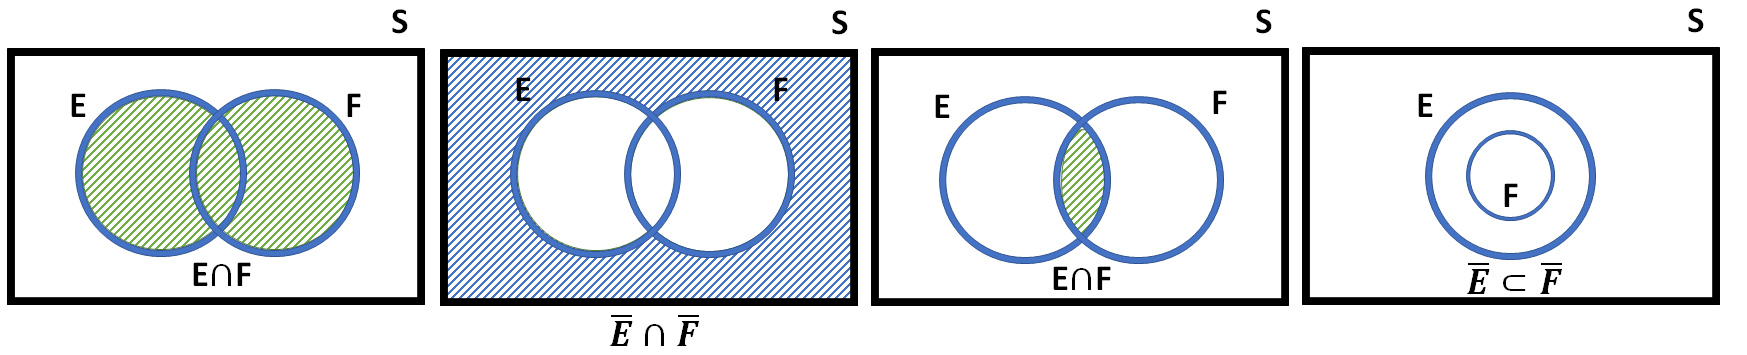
\includegraphics[scale=0.4]{Setrepresentation.png}
		 \end{figure}
		 \item \textbf{Permutations($^nP_r$)}
		 	\begin{itemize}
		 		\item Permutation means \textbf{Arrangement} $\boxed{^nP_r = \dfrac{n!}{(n-r)!}} \impliedby$ (Ways to arrange r things out of n things)
		 	\end{itemize}
		 \item \textbf{Combinations($^nC_r$)}
		 	\begin{itemize}
		 		\item Combination means \textbf{Selection} $\boxed{^nC_r = \dfrac{n!}{(n-r)!r!} = \dfrac{^nP_r}{r!}}\impliedby$ (Ways to select r things out of n things)
		 	\end{itemize}
	\end{itemize}\hrulefill
%-----------------------------------------------------------------------------------------%
	\section{Types of Events}
	\subsection{Complementary events}
		\begin{itemize}
			\item If S=\{1,2,3,4,5\} and A = even numbers - \{2,4\}, then the complimentary even of A is denoted by $\bar{A}$=\{1,3,5\}
		\end{itemize}
%-----------------------------------------------------------------------------------------%
	\subsection{Equally likely events}
		\begin{itemize}
			\item Two events are equally likely events when the probability for both the events are same. For Eg. Getting a head or a tail on a coin toss is 50/50
		\end{itemize}
%-----------------------------------------------------------------------------------------%
	\subsection{Mutually Exclusive events}
		\begin{itemize}
			\item Two events are mutually exclusive if when one event occurs, the other cannot occur simultaneously. For eg. you can get only a head or a tail but not both on a coin toss on a single try.
			\item $\boxed{p(E_1\cup E_2)=p(E_1)+p(E_2)}\impliedby$ ($E_1$ and $E_2$ are mutually exclusive) $\implies\boxed{p(E_1\cap E_2) = 0}$
		\end{itemize}
%-----------------------------------------------------------------------------------------%
	\subsection{Collectively Exhaustive events}
		\begin{itemize}
			\item If the union of two events give the sample space, then they are called collectively exhaustive events
		\end{itemize}
%-----------------------------------------------------------------------------------------%
	\subsection{Independent events}
		\begin{itemize}
			\item When the occurrence of one event doesn't affect the occurrence of another event. For eg. In a bag of 5 red balls and 3 black balls, if two balls are drawn at random one at a time \textbf{with replacement}, then the probability of getting say 2 red balls is not affected by whether you got red ball on the first pick or not. 
			\item If it had been \textbf{without replacement}, then the probability will change
			\item If two events are independent, then conditional probability becomes marginal probability 
			\item $\implies p(A/B) = p(A),\;\;p(B/A) = p(B)\;\;\;\boxed{p(A\cap B) = p(A)*p(B)}$
		\end{itemize}\hrulefill
%-----------------------------------------------------------------------------------------%
\section{De Morgan's Law}
	\begin{itemize}
		\item $\boxed{\overline{(E_1\cup E_2)} = (\bar{E_1}\cap \bar{E_2})}\;\;\;\boxed{(\overline{E_1\cap E_2)} = (\bar{E_1}\cup \bar{E_2})}\;\;\;$ $\boxed{p(\bar{E_1}\cap \bar{E_2})\;i.e.,(\;Neither\;E_1\;nor\;E_2) = 1 - p(E_1\cup E_2)}$
	\end{itemize}\hrulefill
%-----------------------------------------------------------------------------------------%
\section{Approaches to Probability}
	\subsection{Classical Approach}
		\begin{itemize}
			\item $\boxed{p(E) = \dfrac{n(E)}{n(S)}}\impliedby$ (Classical approach assumes that all outcomes are equally likely)
		\end{itemize}\hrulefill
%-----------------------------------------------------------------------------------------%
\section{Rules of Probability}
	\begin{enumerate}
		\item $\boxed{p(A\cup B)=p(A)+p(B)-p(A\cap B)}\impliedby$ \textbf{(Inclusion-Exclusion rule)}
		\item $\boxed{p(A\cup B) = p(A)*p(B/A) = p(B)*p(A/B)\impliedby}$ \textbf{(Conditional Probability)}
			\begin{itemize}
				\item Here, p(A) and p(B) are called \textsc{Marginal probabilities}
				\item p(A/B) and p(B/A) are called \textsc{Conditional probabilities}
				\item p(A/B) = Probability of occurrence of A when B has already occurred
				\item p(B/A) = Probability of occurrence of B when A has already occurred
				\item Conditions for three events A,B,C to be independent:
					\begin{itemize}
						\item \fbox{p(ABC) = p(A)p(B)p(C)} \fbox{p(AB) = p(A)p(B)} \fbox{p(BC) = p(B)p(C)} \fbox{p(AC) = p(A)(C)}
					\end{itemize}
			\end{itemize}
		\item $\boxed{p(A)=1-p(\bar{A})}\;\;\;\boxed{p(A)+p(\bar{A})=1}\impliedby$ \textbf{(Complimentary probability)}
		\item $\boxed{p(A/B)=\dfrac{p(A\cap B)}{p(B)}}\;\;\;\boxed{p(B/A)=\dfrac{p(A\cup B)}{p(A)}}\impliedby$ \textbf{(Conditional probability - multiplication rule)}
		\item $\boxed{p(E) = p(A\cap E)+p(B\cap E) = p(A)*(p(E/A)+p(B)*p(E/B))}\impliedby$ \textbf{(Total probability)}
			\begin{itemize}
				\item If an event E can occur in two ways A and B, then the total probability for the occurrence of E is the sum the probability of it happening by A and the probability of E happening by B.
			\end{itemize}
		\item $\boxed{p\left(E_i/A\right) = \dfrac{p(E_i\cap A)}{A} = \dfrac{p(E_i)*p(E_i/A)}{\sum_{k=1}^{n}p(E_k).p(A/E_k)}} \impliedby$ \textbf{(Baye's Theorem)}
	\end{enumerate}\hrulefill
%-----------------------------------------------------------------------------------------%
\chapter{Statistics}
		\section{Basics and Introduction}
		\begin{itemize}
			\item A branch of mathematics that gives us the means to work with large datasets and derive meaningful results from it
			\item Descriptive measures:
				\begin{itemize}
					\item Measure of Central tendency: indicates the avg value of data
					\item Measure of dispersion: denotes about the extent to which data items deviate from the central tendency value. In other words, "It quantifies the variation in data"
				\end{itemize}\hrulefill
		\end{itemize}
%-----------------------------------------------------------------------------------------%
		\section{Arithmetic Mean($\bar{x}$)}
			\begin{itemize}
				\item $\boxed{\bar{x}=\dfrac{\sum x}{n}}\impliedby$ (for raw data) $\;\;\;\boxed{\bar{x}=\dfrac{\sum (f_ix_i)}{\sum f_i}}\impliedby$ (for Grouped data)
			\end{itemize}\hrulefill
%-----------------------------------------------------------------------------------------%
		\section{Median}
		\subsection{Median for Raw data}
			\begin{itemize}
				\item First arrange the elements in Ascending order
				\item $\boxed{\left(\dfrac{n+1}{2}\right)^{th}term}\impliedby$ (n=odd) $\;\;\;\boxed{\dfrac{\left(\dfrac{n}{2}\right)^{th}term+\left(\dfrac{n}{2}+1\right)^{th}term}{2}}\impliedby$ (n=even)
			\end{itemize}\hrulefill\\\\
%-----------------------------------------------------------------------------------------%
		\subsection{Median for Grouped data}
		\begin{table}[H]
			\centering
			\begin{tabular}{cc}
				\parbox{8cm}{Median = $\boxed{L + \left[\dfrac{\left(\dfrac{N+1}{2}\right)-(F+1)}{f_m}\right]*h}$} & \hspace{-1cm}
				\parbox{9cm}{L = Lower limit of median class\\\\N = Total number of data items = $\sum F$\\\\ F = cumulative frequency of the class immediately preceding the median class\\\\$f_m$ = Frequency of the median class\\\\h = width off the median class}
			\end{tabular}
		\end{table}\hrulefill
		\begin{itemize}
			\item Consider the following example for calculation of Median in grouped data:
			\begin{table}[H]
				\centering
				\def\arraystretch{1.5}
				\begin{tabular}{|c|c|c|}
				\hline
				\textbf{Mark Range} & \textbf{f (No. of students)} & \textbf{Cumulative frequency}\\
				\hline
				(00-20) & 02 & 02\\
				\hline
				(21-40) & 03	& 05\\
				\hline
				(41-60) & 10	& 15\\
				\hline
				(61-80) & 15	& 30\\
				\hline
				(81-100) & 20	& 50\\		
				\hline	
				\end{tabular}							
			\end{table}
			\item In the above example, $\left(\dfrac{N+1}{2}\right)$ = $\dfrac{(2+3+10+15+20)+1}{2} = 25.5$
			\item Class (61-80) is the median class as $30 > 25.5$
			\item Here, \fbox{L=61} \fbox{h=20} \fbox{F=15} $\boxed{f_m=15}$\hspace{1cm}So, Median = $60 + \dfrac{25.5-(15+1)}{15} * 20$ = 69.66 $\approx$ 69.7
		\end{itemize}\hrulefill
%-----------------------------------------------------------------------------------------%
	\section{Mode}
		\begin{itemize}
			\item Mode is the value that occurs most frequently in the data. If more than one data is occuring most frequently, then both of them are mode.
		\end{itemize}
		\subsection{Mode of Raw data}
			\begin{itemize}
				\item Found using observation
			\end{itemize}\hrulefill
%-----------------------------------------------------------------------------------------%
		\subsection{Mode of Grouped data}
			\begin{table}[H]
				\centering
				\def\arraystretch{1.5}
				\begin{tabular}{cc}
					\parbox{4cm}{$\boxed{Mode = L+\dfrac{f_0-f_1}{2f_0-f_1-f_2}*h}$} & \hspace{1cm}
					\parbox{10cm}{L = Lower limit of the modal class\\$f_0$ = Modal frequency i.e. Largest frequency\\$f_1$=Frequency in the class preceding the modal class\\$f_2$ = Frequency in the class succeeding the modal class\\h = width of the class}
				\end{tabular}
			\end{table}
			\begin{itemize}
				\item Consider the following example for calculation of Mode in grouped data:
			\end{itemize}
			\begin{table}[H]
				\centering
				\def\arraystretch{1.5}
				\begin{tabular}{|c|c|}
					\hline
					\textbf{Height(in ft)} & \textbf{Number of students}\\
					\hline
					3.0 - 3.5 & 12\\
					\hline
					3.6 - 4.0 & 37\\
					\hline
					4.1 - 4.5 & 79\\
					\hline
					4.6 - 5.0 & 152\\
					\hline
					5.1 - 5.5 & 65\\
					\hline
					5.6 - 6.0 & 7\\
					\hline
					\textbf{Total} & 352\\
					\hline
				\end{tabular}
			\end{table}
			\begin{itemize}
				\item Since, 152 is the largest frequency, the modal class is (4.6 - 5.0)
				\item Thus, \fbox{L=4.6} $\boxed{f_0 = 152}$ $\boxed{f_1 = 79}$ $\boxed{f_2 = 65}$ \fbox{h = 0.5}\hspace{1cm} Mode = $4.5 * \dfrac{152 - 79}{2(152) - 79 - 65}*0.5 \approx 4.73$
			\end{itemize}\hrulefill
%-----------------------------------------------------------------------------------------%
	\section{Properties relating Mean, Median and Mode}
		\begin{itemize}
			\item When an approx value of mode is required: $\boxed{Emprical\;mode = 3*(Median)-2*(Mean)}$
			\begin{figure}[H]
				\centering
				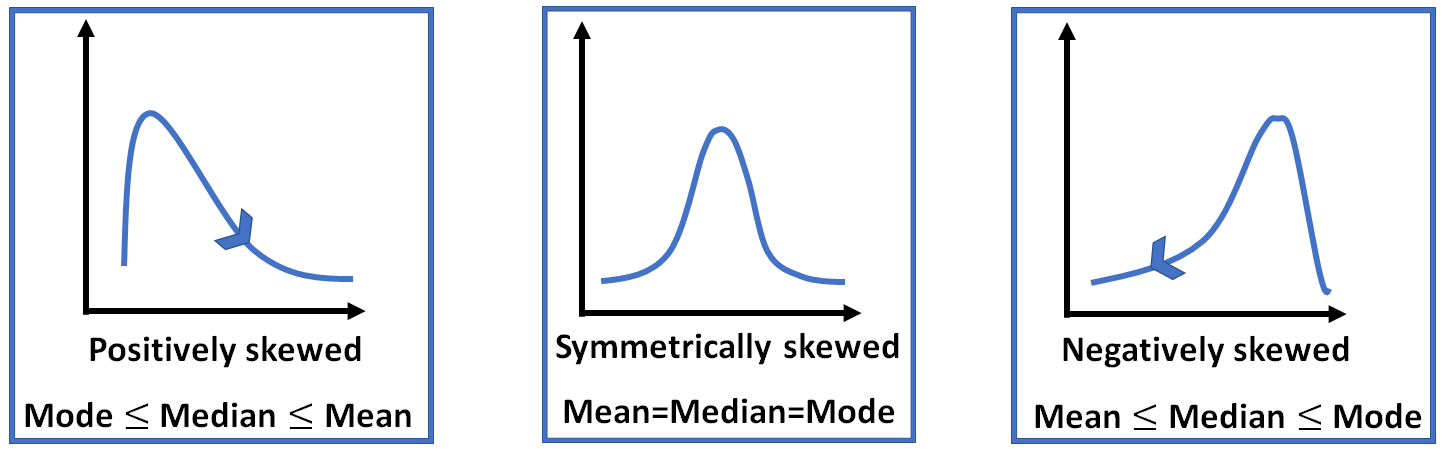
\includegraphics[scale=0.4]{MeanMedianModeRelation.png}
			\end{figure}
		\end{itemize}\hrulefill
%-----------------------------------------------------------------------------------------%
	\section{Standard Deviation and Variance}
	\subsection{Standard Deviation for RAW data}
		\begin{itemize}
			\item It is a measure of variation among the data
			\item Consider there are five values: $x_1,x_2,x_3,x_4,x_5$ The mean $\bar{x} = \dfrac{x_1+x_2+x_3+x_4+x_5}{5}$.
			\item The individual deviations are ($x_1-\bar{x}),\;(x_2-\bar{x}),\;(x_3-\bar{x}),\;(x_4-\bar{x}),\;(x_5-\bar{x})$
			\item \textbf{Variance($\sigma^2$)} = Mean of Square of each deviation of data = $\boxed{\sigma^2 = \dfrac{\sum _{i=1}^n(x_i-\bar{x})^2}{n}}$
			\item \textbf{Standard deviation($\sigma$)} = $\boxed{\sqrt{Variance} = +\sqrt{\dfrac{\sum _{i=1}^n(x_i-\bar{x})^2}{n}}}$
		\end{itemize}\hrulefill
%-----------------------------------------------------------------------------------------%
	\subsection{Standard Deviation for Grouped data}
		\begin{itemize}
			\item $\boxed{Arithmetic\;Mean(\bar{x})=\dfrac{\sum (f_ix_i)}{\sum f_i}}\;\;\;\boxed{Variance(\sigma^2) =\sum _{i=1}^{n}\left(\dfrac{f_i(x_i - \bar{x})^2}{f_i}\right)}$ 
		\end{itemize}\hrulefill
%-----------------------------------------------------------------------------------------%
	\section{Coefficient of Variation}
		\begin{itemize}
			\item The standard deviation is an absolute measure of variation and hence cannot be used for comparison of variation between 2 different data sets with different mean.
			\item For the above purpose a relative measure of variation called, \textbf{Coefficient of Variation(CV)} is used. $\boxed{CV =\dfrac{\sigma}{\bar{x}}}$. CV is often represented as a percentage
		\end{itemize}\hrulefill
%-----------------------------------------------------------------------------------------%
	\section{Probability Distribution}
		\subsection{Random Variable}
			\begin{itemize}
				\item It is a real valued function. 
				\item For eg. Tossing 3 coins. x be the real valued function denoting the number of heads. 
				\begin{table}[H]
					\centering 
					\def\arraystretch{1.5}
					\begin{tabular}{|c|c|c|c|c|}
						\hline
						x & 0 & 1 & 2 & 3\\
						\hline
						p(x) & 1/8 & 3/8 & 3/8 & 1/8\\
						\hline 
					\end{tabular}	
				\end{table}
				\item It is of two types: Discrete and Continuous
			\end{itemize}\hrulefill
%-----------------------------------------------------------------------------------------%
		\subsection{Discrete Random Variable}
			\begin{itemize}
				\item eg. x = function representing the possible sum of values of two fair dice. 
				\item x can have only discrete values of any one of \{2,3,4,5,6,7,8,9,10,11,12\}
			\end{itemize}\hrulefill
%-----------------------------------------------------------------------------------------%
		\subsection{Continuous Random Variable}
			\begin{itemize}
				\item eg. x = function representing the volume of a water in a container
				\item In this case, x can have any value between 0 to the volume.
			\end{itemize}\hrulefill
%-----------------------------------------------------------------------------------------%
		\subsection{Probability Density Function(F(x))}
			\begin{itemize}
				\item $\boxed{F(x) \geq 0}\;\;\;\boxed{\int_{-\infty}^\infty F(x)dx= 1}\;\;\;\boxed{p(a<x<b)=\int_a^bF(x)dx}$
				\item In simple terms, it tells us the likelihood of a continuous random variable having a value between any two points, rather than having a specific value as in the case of a discrete random variable. 
				\item The pdf assigns a value between 0 and 1 to every possible value of the continuous random variable, such that the integral of the pdf over the entire range of the random variable is equal to 1. 
				\item This means that the area under the curve of the pdf represents the total probability of the random variable being in that range of values.
			\end{itemize}\hrulefill
%-----------------------------------------------------------------------------------------%
		\subsection{Probability Mass Function(p(x))}
			\begin{itemize}
				\item $\boxed{p(x) = P[X=x]}\;\;\;\boxed{p(x)\geq 0}\;\;\;\boxed{\sum p(x)=1}$
				\item In simple terms, it gives the exact probability of a discrete random variable having a specific value. The PMF assigns a probability between 0 and 1 to each possible value of the discrete random variable such that the sum of the probabilities for all possible values is equal to 1. 
				\item In other words, the PMF gives the probability distribution of a discrete random variable and allows us to see the likelihood of each possible outcome.
			\end{itemize}\hrulefill
%-----------------------------------------------------------------------------------------%
	\section{Distributions}
		\begin{itemize}
				\item Distributions are also of two types based on the above:
					\begin{itemize}
						\item Discrete distribution: Poisson, Hypergeometric
						\item Continuous distribution: Uniform, Normal and Exponential
					\end{itemize}
		\end{itemize}\hrulefill
%-----------------------------------------------------------------------------------------%
		\subsection{Properties of Discrete Distribution}
			\begin{itemize}
				\item $\boxed{\sum P(x) = 1}\;\;\boxed{E(x)=\sum xp(x)}\;\;\boxed{V(x)=E(x^2)-(E(x))^2}$ (E(x) = Expected value, V(x) = Variance of RV)
			\end{itemize}\hrulefill
%-----------------------------------------------------------------------------------------%
		\subsection{Properties of Continuous Distribution}
			\begin{itemize}
				\item $\boxed{\int_{-\infty}^\infty f(x)dx = 1}\;\;\boxed{F(x) = CDF = \int_{-\infty}^x f(x)dx}\;\;\boxed{E(x) = \int_{-\infty}^\infty xf(x)dx}$
				\item CDF = Cumulative Distribution Function.
				\item CDF gives us the cumulative probability of a random variable being less than or equal to a certain value, while the PDF gives us the likelihood of a random variable taking on a specific value within a certain range.
				\item $\boxed{p(a<x<b)=p(a\le x<b)=p(a<x\le b)=p(a\le x\le b)=\int_a^b f(x)dx}$
			\end{itemize}\hrulefill
%-----------------------------------------------------------------------------------------%
		\subsection{Properties of Expectation(E(x)) and Variance(V(x))}
			\begin{itemize}
				\item $\boxed{E(c)=c}\;\;\boxed{V(c)=0}\;\;\boxed{E(cx)=cE(x)\implies E(-x)=-E(x)}\impliedby$ (c = constant)
				\item $\boxed{V(cx)=c^2V(x)\implies V(-x)=(-1)^2V(x)=V(x)}\;\;\boxed{V(c_1x_1+c_2x_2)=c_1^2V(x_1)+c_2^2V(x_2)+2c_1c_2cov(x_1,x_2)}$
				\item If ($x_1,x_2$) are independent variables, then $cov(x_1,x_2)=0$
				\item $\boxed{V(x_1+x_2)=V(x_1-x_2)=V(x_1)+V(x_2)}$
				\item $\boxed{E(X+Y)=E(X)+E(Y)}\impliedby$ (X,Y are two random variables)
				\item $\boxed{E(XY)=E(x)E(Y)}\;\;\boxed{V(X+Y)=V(X)+V(Y)}\impliedby$ (X,Y are two independent Random Variables)
			\end{itemize}\hrulefill
%-----------------------------------------------------------------------------------------%
	\section{Discrete Distributions}
		\subsection{General Discrete Distribution}
			\begin{itemize}
				\item Let X be the number which comes on a single throw of dice. The probability distribution table is given by
				\begin{table}[H]
					\centering
					\def\arraystretch{1.5}
					\begin{tabular}{|c|c|c|c|c|c|c|}
						\hline
						x & 1 & 2 & 3 & 4 & 5 & 6\\
						\hline
						p(x) & 1/6 & 1/6 & 1/6 & 1/6 & 1/6 & 1/6\\
						\hline 
					\end{tabular}
				\end{table}
				\item For this case, p(x) for all x is same. But this will not be the case always. 
				\item But, $\sum p(x) = 1$ always
				\item From the above table, we can easily calculate E(x), V(x).
				\item E(x) is the expected value of x and is similar to the average value of x after infinite trials. So E(x) is sometimes written as $\mu_x$
				\item V(x) represents the variability of X. So it is written sometimes as $\sigma_x^2$	
				\item $\boxed{cov(x,y)=E(xy)-E(x)E(y)}\;\;\boxed{cov(x,y)=0}\impliedby$ (If x,y are independent Random variables)											
			\end{itemize}\hrulefill
%-----------------------------------------------------------------------------------------%
		\subsection{Binomial Distribution (n,p)}
			\begin{itemize}
				\item Consider a trial experiment of n independent trials
				\item each of which will result in success with probability p or failure with probability 1-p
				\item If X represents the number of successes that occur in the n trials, then X is the Binomial Random variable with parameters (n,p)
				\item Conditions to be satisfied for Binomial distribution:
					\begin{itemize}
						\item Only 2 outcomes are possible: success or failure
						\item The probability of outcome should remain same from trial to trial
						\item The outcome of one trial should not affect the outcome of another. 
					\end{itemize}
				\item Then the probability of obtaining x successes from n trials is given by:
$\boxed{p(X=x)= (^nC_x)p^x(1-p)^{n-x}}$
				\item Here, $\boxed{E(X)=np}\;\;\boxed{V(x)=np(1-p)}$
				\item By \textbf{Recurrence relation:} $\boxed{p(X=(x+1)) = \dfrac{(n-x)p}{(n+x)(1-p)}p(x)}$
			\end{itemize}\hrulefill
%-----------------------------------------------------------------------------------------%
		\subsection{Hypergeometric Distribution}
			\begin{itemize}
				\item If probability changes from trial to trial, then one condition of the binomial distribution is violated. In such a case, Hypergeometric distribution is used. \textbf{Mainly used in case of sampling without replacement from a finite population}
				\item For eg. Consider the situation:
					\begin{itemize}
						\item There are 10 markers on a table - 6 are defective(D), 4 are NonDefective(ND)
						\item 3 are randomly taken without replacement
						\item Find the probability of exactly one marker being defective
					\end{itemize}
				\item Since it is without replacement, after each draw(trial), the probability will change. 
				\item Solution: Let X denote the num of defective marker. $\implies\boxed{p(X=x)=\dfrac{(^6C_x)(^4C_{3-x})}{^10C_3}}$
				\item With the above formula for the above problem, we can easily now find the solution as well find other solutions like: At least one marker being defective $\implies (p(X=(x\geq 1)) = p(X=0)+p(X=1))$\\\\
				\textsc{Generalized formula for Hypergeometric distribution:}
				\begin{itemize}
					\item Consider n objects of with r are of type 1 and (n-r) are of type 2. From this w objects are drawn.
					\item[] $$\boxed{p(X=x)=\dfrac{(^rC_x)(^{n-r}C_{w-x})}{^nC_w}}\;\;\boxed{E(x)=n*\left(\dfrac{r}{n}\right)}$$
				\end{itemize}
			\end{itemize}\hrulefill
%-----------------------------------------------------------------------------------------%
		\subsection{Geometric Distribution (p)}
			\begin{itemize}
				\item \textbf{Consider an experiment to be performed until successes is obtained} 
				\item let the probability of success be p and probability of failure be (1-p)=q
				\item let x denote the number of times the experiment has to be repeated to obtain success
				\item The distribution of random variable x is given by:
				\begin{table}[H]
					\centering
					\def\arraystretch{1.5}
					\begin{tabular}{|c|c|c|c|c|c|}
						\hline
						k & 1 & 2 & 3 & 4 & ...\\
						\hline
						p(k) & $q^0p$ & $q^1p$ & $q^2p$ & $q^3p$ & ....\\
						\hline
					\end{tabular}
				\end{table}
				\item $\boxed{p(k) = p(x-k) = q^{k-1}p}\;\;\boxed{E(x) = 1/p}\;\;\boxed{V(x)=\dfrac{q}{p^2}}\;\;\boxed{CD = F(k)=-1-q^k}\;\;\boxed{p(x>r)=q^r}$
			\end{itemize}\hrulefill
%-----------------------------------------------------------------------------------------%
		\subsection{Poisson Distribution($\lambda$)}
			\begin{itemize}
				\item $\pmb{\lambda}$ \textbf{= average number of occurrences of event in an observation period} $\pmb{\Delta t}\implies \boxed{\lambda = \alpha\Delta t}$ 
				\item $\alpha \implies$ number of occurrence of event per unit time
				\item $\boxed{p(x=x)=\dfrac{e^{-\lambda}\lambda^x}{x!}}\;\;\;\;\;\boxed{p(x=(x+1)) = \dfrac{\lambda}{x+1}p(x)}\impliedby$ (Recurrence relation) (obtained by p(x)/p(x+1))
				\item \textbf{NOTE: } Poisson distribution is used to approximate Binomial distribution when n is very large and p is very small for binomial distribution. So we'll use $\boxed{\pmb{\lambda = np}}$
			\end{itemize}\hrulefill
%-----------------------------------------------------------------------------------------%
	\section{Continuous Distribution}
		\subsection{General Continuous Distribution}
			\begin{itemize}
				\item
			\end{itemize}\hrulefill
%-----------------------------------------------------------------------------------------%		
		\subsection{Uniform Distribution}
			\begin{itemize}
				\item
			\end{itemize}\hrulefill
%-----------------------------------------------------------------------------------------%
		\subsection{Exponential Distribution}
			\begin{itemize}
				\item
			\end{itemize}\hrulefill
%-----------------------------------------------------------------------------------------%
		\subsection{Normal Distribution}
			\begin{itemize}
				\item
			\end{itemize}\hrulefill
%-----------------------------------------------------------------------------------------%
		\subsection{Standard Normal Distribution}
			\begin{itemize}
				\item
			\end{itemize}\hrulefill
%-----------------------------------------------------------------------------------------%
\chapter{Numerical Methods}
%-----------------------------------------------------------------------------------------%
\chapter{Complex Numbers}
%-----------------------------------------------------------------------------------------%
\chapter{Transform Theory}
%-----------------------------------------------------------------------------------------%
%-----------------------------------------------------------------------------------------%
\end{document}
%-----------------------------------------------------------------------------------------%
%-----------------------------------------------------------------------------------------%
%-----------------------------------------------------------------------------------------%
